% Metódy inžinierskej práce

\documentclass[10pt,oneside,slovak,a4paper]{article}

\usepackage[slovak]{babel}

\usepackage[IL2]{fontenc} 
\usepackage[utf8]{inputenc}
\usepackage{graphicx}
\usepackage{url} 
\usepackage{hyperref} 

\usepackage{cite}

\usepackage{graphicx}
\usepackage{subcaption}



\title{Fungovanie umelej inteligencie v hrách\thanks{Semestrálny projekt v predmete Metódy inžinierskej práce, ak. rok 2022/23}} % meno a priezvisko vyučujúceho na cvičeniach

\author{Matúš ILLITH\\[2pt]
	{\small Slovenská technická univerzita v Bratislave}\\
	{\small Fakulta informatiky a informačných technológií}\\
	{\small \texttt{xillith@stuba.sk}}
	}

\date{\small 13.decembra.2022} 



\begin{document}

\maketitle

\begin{abstract}
\ldots



Umelá inteligencia je súčasťou herného sveta od nepamäti. Od prvých arkádových hier, ako Pac-Man kde umelá inteligencia ovládala duchov a vytvárala pre nás hráčov pocit napätia. Avšak umelá inteligencia sa nedá vyjadriť iba jedným kódom. V dnešnej dobe silné umelé inteligencie využívajú techniku kedy učia stroje, ako sa majú správať.

Pri prvých hrách táto možnosť neexistovala využívali sa rôzne druhy rozhodovania, ako napríklad rozhodovanie podľa pravidiel, stavový automat a samozrejme riadenie podľa skrípt, ktoré sa využívalo v hernej klasike Pac-Man. Pri vývoji Pac-Mana a jeho umelej inteligencie, ktorá riadi duchov vznikali rôzne problémy. Niektoré tieto chyby sa dostali aj do finálnej verzie hry ktorú každý z nás určite hral. Napríklad duchovia sa nesprávajú podľa svojich pravidiel keď sa Pac-Man pozerá hore.

Umelá inteligencia spravila obrovský posun za posledných niekoľko rokov ale netreba zabúdať na začiatky bez ktorých by sme dneska nedokázali hrať naše obľúbene hry či už to je Pac-Man, Halo alebo aj šach.
\end{abstract}
\newpage
\tableofcontents
\newpage

\section{Úvod}




Svet si pod pojmom umelá inteligencia predstaví takmer vždy len tú v hernej podobe. Umelá inteligencia sa však nenachádza len v hrách. Nie je pochýb, že bez umelej inteligencie by dnešný svet nedokázal fungovať. Je jednou z najpodstatnejších časti každej technológie, i keď si to na prvý pohľad neuvedomujeme. Nachádza sa v mobiloch, kde umelá inteligencia (neskoršie iba AI) rozhoduje, koľko výkonu procesora si môže aplikácia zobrať podľa toho, ako často ju používame. Nájsť ju však môžeme napríklad v satelitoch, v inteligentných domácnostiach a podobne. Najdôležitejšou časťou umelej inteligencie je stále však jej využitie v hrách. Sprevádza herný svet od jeho počiatkov, je jednou z hlavných častí hrania. Posúva hráčov k bádaniu, ktorí vďaka nej sú schopní dávať podnet k posunu dopredu a vymýšľať nové riešenia.
Čo je teda tá umelá inteligencia?~\ref{def1}




\section{Definícia AI} \label{def1}

Definícia umelej inteligencie podľa IBM:
"Umelá inteligencia využíva počítače a stroje na napodobňovanie schopností ľudskej mysle riešiť problémy a vykonávať rozhodovania."
Zatiaľ čo v posledných desaťročiach sa objavilo niekoľko definícií umelej inteligencie (AI), John McCarthy ponúka nasledujúcu definíciu: "Je to veda a inžinierstvo výroby inteligentných strojov, najmä inteligentných počítačových programov. Súvisí to s používaním počítačov na porozumenie ľudskej inteligencie, bez toho aby sa umelá inteligencia viazala na biologické nedostatky ľudskej mysle." 

Niekoľko rokov pred touto definíciou sa Alan Turing v jeho seminárnej práci z roku 1950 spýtal zaujímavú otázku:"Vedia počítače myslieť? ". Kvôli tejto otázke vytvoril dnes dobre známy " Turing test". V tomto teste sa človek snaží zistiť, či odpovede na otázky boli vytvorené počítačom alebo človekom. Zatiaľ čo verejnosť má silné myšlienky proti tomuto test nieje pochýb o tom, že je jednou z časti histórie umelej inteligencie. ~\cite{3.zdroj}



\section{Fungovanie AI} \label{hlavna cast}

Na to aby sme vedeli rozdeliť rôzne myšlienkové pochody umelej inteligencie v hrách, treba si povedať kde všade sa v hrách AI nachádza.
V hrách sa stretávame s rôznymi typmi umelej inteligencie, od najznámejšie umelej inteligencie, ktorá napodobňuje správanie ľudí, zvierat a často sprevádza hráča novými miestami takzvané NPC (Non-playable character), až po umelú inteligenciu, ktorá vytvára a riadi celý náš herný svet. 
~\cite{1.zdroj}

Práve na tieto typi umelej inteligencie, vieme priradiť rôzne druhy rozhodovania:
\vspace{0.5cm}
\subsection{Riadenie podľa pravidiel}

Riadenie podľa systému pravidiel sa považuje za jedno z najstarších foriem rozhodovanie. Využíva sa hlavne pre správanie dynamických objektov v arkádach.
Tento systém sa najčastejšie používa keď máme malý počet entít a zložitejší reťazec podmienok. Keď dôjde na koniec reťazca spustí sa konkrétny skript na vykonanie určitej akcie.~\ref{skript}

Riadenie podľa systému pravidiel vieme znázorniť tabuľkou, kde v poslednom stĺpci sa nachádza akcia ktorú má daná entita splniť. V ostatných stĺpcov sa nachádzajú podmienky, ktoré zapríčinia túto akciu.~\ref{fig:rbs.1}. Jedným z príkladov sú vojenské jednotky kontrolované AI , kde sú určene priority čo musí daná jednotka spraviť.

Ak má malo oleja musí ho najprv vyťažiť. Potom ak má málo energie musia si postaviť elektrárňu a keď im chýbajú vojaci musia regrutovať vojakov. Ak majú všetko splnené tak potom zaútočia.



\begin{figure} [h!]
  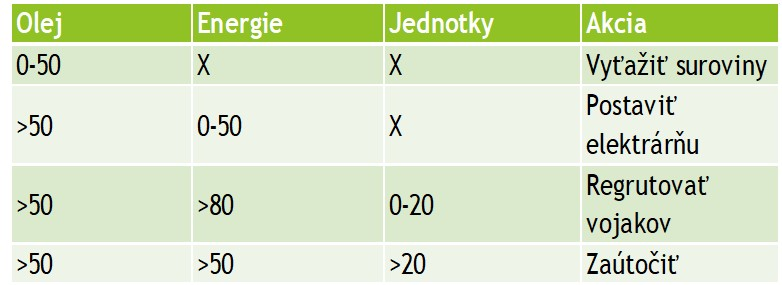
\includegraphics[scale=0.7]{tabulka2.jpg}
  \caption{Dvojrozmerná tabulka. Zdroj: vlastná výroba autora}
  \label{fig:rbs.1}
\end{figure}



\subsection{Riadenie podľ skrípt} \label{skript}

Riadenie skriptami sa považuje za jedno z najjednoduchších foriem riadenia entít. Jeden z najlepších príkladov je hra Pac-Man. V hre Pac-Man sú duchovia kontrolovaný AI, ako jediná entita v celej hre. Duchovia sa riadia zložitejšími skriptami, ktoré článok preberá neskoršie.~\ref{Pac-Man}.

Taktiež dokážeme skriptami riadiť rôzne objekty aby menili svoje správanie. 


\subsection{Stavový automat} \label{FSM}

Stavový automat sa nachádza pri vyžití if-this-than-that procesu. Entita sa nachádza v stavoch dopredu definovaných kedy sa má spustiť stavový automat(neskoršie iba :FSM). Po aktivácii sa daný stav zmení. Každá situácia sa môže teda reprezentovať skriptom alebo ďalším FSM. Entita sa môže nachádzať vo  viacerých stavoch naraz. Ak sa tak stane využíva sa hierarchicky FSM kde každý stav ma ďalšie podstavy.

FSM vieme graficky znázorniť tak, že každý vrchol grafu ukazuje stav, v akom sa entita nachádza a každá hrana predstavuje akciu, ktorá sa vykonáva a mení dané stavy.~\cite{1.zdroj}
\begin{figure} [h!]
  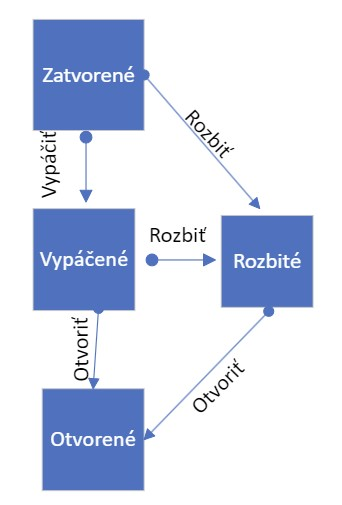
\includegraphics[scale=0.43]{stv2.jpg}
  \caption{Grafové znázornenie FSM pre okno Zdroj:vlastná výroba autora}
  \label{fig:FSM}
\end{figure}

\newpage
\subsection{Cieľovo orientované správanie} \label{GDB}

Cieľovo orientované správanie (GDB) používa na definovanie správania úlohy. Úlohy môžu byť atomické kedy ja daná jedna úloha (napr. miešaj nápoj). Keď spojíme viacej takýchto úloh vzniká plán(napr. miešaj nápoj, choď domov, vyspi sa, vstaň, choď do roboty, miešaj nápoj). GDB vieme znázorniť taktiež grafom.

Spojením viacerých úloh vzniká stromový graf kde úlohy tvoria listy. Každý plán sa dá rozdeliť na základné úlohy. Potom tento plán sa dá rozdeliť na sekvenčný, plán kde pokiaľ sa nespravia všetky úlohy tak plán nebol spravený, alebo selekčný plán, tam stačý aby sa spravila jedna podmienka aby sa plán splnil. ~\cite{1.zdroj}


\subsection{Strom správania} \label{BT}

Tento spôsob je jedným z najobľúbenejších spôsobov správania ktoré vývojári implementujú do svojich hier.  Vznikol v dvadsiatom prvom storočí a prvý krát sa ukázal v hre Halo2.

 Strom správania reprezentuje mozog NPC. 
Strom správania sa dá reprezentovať stromovým grafom. Listy stromu predstavujú  čiastočnú akciu a vnútorne uzly vytvárajú rozhodovací impulz.~\cite{1.zdroj}


\section{Porozumenie spravnia duchov v hre Pac-Man}\label{Pac-Man}

\subsection{Priebeh hry}\label{ph}



V hre Pac-Man sú duchovia hlavným oponentom pre nás hráčov. Hráč sa im musí vyhýbať aby zjedol všetky guľôčky a mohol ďalej postupovať v hre. Každý duch v hre má svoju vlastnú osobnosť. Táto osobnosť predstavuje práve to, ako sa daný duch počas hry pohybuje. O tomto pohybe práve rozhoduje AI.


Na začiatku sa hráč ocitne v bludisku ktorého rozloženie sa počas hry nemení. Každým levelom sa však z časti mení správanie duchov a ich rýchlosť. Taktiež sa mení i rýchlosť Pac-Mana.Avšak po level 21 sa nemení žiaden iný parameter. Pac-Man musí pozbierať 240 guľôčok pričom z čoho sú 4 nabité a dovolia Pac-Manovy zjesť duchov. Duchovia začínajú v domčeku do ktorého Pac-Man nemá prístup. Z domčeka počas hry postupne vychádzajú a vrátia sa tam až po tom čo ich Pac-Man zje.
\begin{figure}[h!]
  \centering
  \begin{subfigure}[b]{0.4\linewidth}
    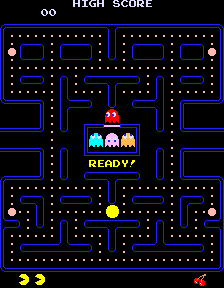
\includegraphics[scale=0.35]{pacman start.png}
    \caption{Hracia plocha }\cite{2.zdroj}
  \end{subfigure}
  \begin{subfigure}[b]{0.4\linewidth}
    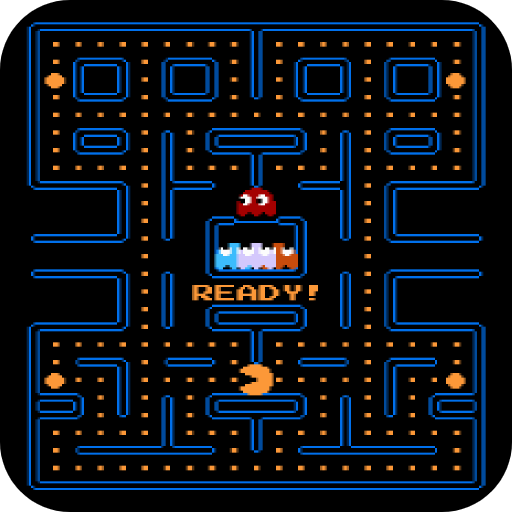
\includegraphics[scale=0.2]{retro pacman.png}
    \caption{Retro hracia plocha.}
  \end{subfigure}
\end{figure}

\subsection{Cieľové dlaždice}
AI v hre Pac-Man sa rozhoduje podľa takzvaných cieľových dlaždíc. AI rozdelí celé bludisko do menších štvorčekov, ktoré majú veľkosť 8 x 8 pixelov, ktoré predstavujú pozície na ktorých sa entity nachádzajú. Duch zje Pac-Mana v tedy keď zaberajú rovnakú dlaždicu, lenže model Pac-Mana a duchov je väčší, ako dané dlaždice preto sa v hre berie len stred modelov. Ak stredy modelov zaberajú rovnakú dlaždicu tak v tedy nastáva určitá reakcia či už Pac-Man zjedol ducha alebo naopak.~\ref{fig:cd}\cite{2.zdroj}
\begin{figure} [h!]
  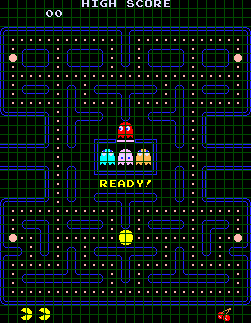
\includegraphics[scale=0.36]{cielove dlazdice.png}
  \caption{Cielové dlaždice}
  \label{fig:cd}
\end{figure}

\subsection{Rôzne správanie duchov}
Duchovia sa nachádzaju vždy v jednom z troch druhov správania.
\begin{enumerate}
    \item Prenasledovť
    \item Roztrúsiť
    \item Báť sa
\end{enumerate}
Keď je duch v režime, kedy prenasleduje Pac-Mana, tak AI využíva takzvané cieľove dlaždice na určenie pozície Pac-Mana a pozície, kam má každý duch ísť. Túto pozíciu má každý duch vlastnú.
Ak duch príde do režimu roztrúsiť, tak pôjde do svojho rohu bludiska, kde sa bude pohybovať.
Duch sa vie dostať do režimu kedy sa bojí iba v tedy, keď Pac-Man zje nabitú guľôčku. Vtedy duch nemá žiadnu dlaždicu na ktorú pôjde, jeho pohyb je úplne náhodný pri každej križovatke. Dĺžka efektu je každým levelom nižšia, až pokým úplne nezanikne v leveli 19.

\subsection{Indviduálne správanie duchov}
Na to aby sme dokázali úplne porozumieť, ako sa duchovia v hre správajú, musíme brať do úvahy, že AI, ktorá riadi duchov je krátkozraká. Duchovia plánujú svoj pohyb iba o jeden krok do budúcnosti. Vždy keď duch príde na novú dlaždicu, tak sa rozhodne na ktorú ďalšiu dlaždicu by sa mal posunúť, a zároveň sa rozhodne kam by sa mal otočiť keď tam príde. 

Tieto rozhodovanie však majú aj svoje zábrany. Napríklad duch sa nikdy nevráti na dlaždicu z ktorej prišiel. Aj keď výnimkou tohto pravidla je keď sa menia režimy z prenasledovania alebo roztrúsenia na hocijaký iný mód. Pri tomto prípade je prinútený vrátiť sa hneď, ako príde na ďalšiu dlaždicu. Tento príkaz prepíše hocijaké rozhodnutie, ktoré AI vytvorila. Toto slúži, ako indikátor pre hráča, že sa zmenili režimy správania, lebo iba pri tomto prípade, sa duch vráti na predchádzajúcu dlaždicu.\cite{2.zdroj}

Každý duch má vlastné meno a prezývku.
\begin{enumerate}
    \item Červený duch sa volá Shadow a jeho przívka je Blinky~\ref{cerv}
    \item Ružový duch sa vola Speedy a jeho przívka je Pinky\ref{pink}
    \item Tyrkysový duch sa vola Bashful a jeho przívka je Inky\ref{Inky}
     \item Oranžový duch sa volá Pokey a jeho prezývka je Clyde\ref{or}
\end{enumerate}

\subsubsection{Červený duch (Blinky)}\label{cerv}
Červený duch je prvé nebezpečenstvo pre Pac-Mana. Blinky začína hru mimo domčeka duchov a hneď po začatí ide do svojho rohu bludiska. Jeho cieľová dlaždica je vždy presná pozícia Pac-Mana.
\begin{figure} [h!]
  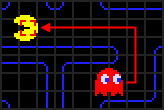
\includegraphics[scale=0.6]{blinky-targeting.png}
  \caption{Červený duch}
  \cite{2.zdroj}
\end{figure}
Aj keď Blinkyho metóda phybu je primitívna má par skrytých trikov. V dopredu definovaných bodoch (vždy podľa zostávajúceho počtu guličiek) sa jeho rýchlosť zvýši o 5 percent a jeho pohyb v režime roztrúsenia sa zmení. Zmena v móde rotrúsenia spočíva v tom, že namiesto toho aby išiel do svojho rohu bludiska, Blinky bude prenasledovať Pac-mana. V podstate bude vždy v móde prenasledovania

\subsubsection{Ružový duch(Pinky)}\label{pink}
Pinky začína hru v domčeku. Pinky sa nehýbe rýchlejšie, ako ostatný duchovia. Dokonca je pomalší, ako Blinky. Aj keď je pomalší, ako Blinky AI sa snaží vybrať jeho cieľovú dlaždicu podľa toho, kde sa Pac-Man pravdepodobne bude nachádzať. AI sa pozerá na aktuálnu pozíciu Pac-Mana a vyberá cieľovú dlaždicu 4 dlaždice pred Pac-Manom. Toto ale fungovalo len keď sa Pac-Man pozeral dole, vľavo alebo vpravo. Keď sa Pac-Man pozeral hore vznikla chyba v kóde, ktorá spravila to, že cieľová dlaždica bola 4 dlaždice pred Pac-Manom a 4 dlaždice vľavo od Pac-Mana.\cite{4.zdroj}
\begin{figure}[h!]
  \centering
  \begin{subfigure}[b]{0.4\linewidth}
    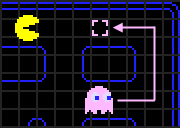
\includegraphics[scale=0.75]{pinky-targeting.png}
    \caption{PInkyho cieľova dlaždica.}
\cite{2.zdroj}
  \end{subfigure}
  \begin{subfigure}[b]{0.5\linewidth}
    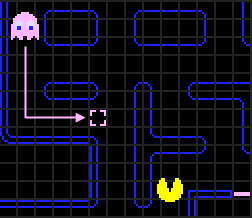
\includegraphics[scale=0.5]{pinky-targeting2.png}
    \caption{Pinkyho chybná cieľová dlaždica.}
\cite{2.zdroj}
  \end{subfigure}
\end{figure}

\subsubsection{Tyrkysový duch(Inky)}\label{Inky}
Inky je jediný duch, ktorý využíva iné špecifika okrem pozície Pac-Mana. Inky používa na určenie cieľovej dlaždice pozíciu a orientáciu Pac-mana a taktiež Blinkyho pozíciu. Na to aby sme našli Inkyho cieľovú dlaždicu musíme sa najprv pozrieť 2 dlaždice pred Pac-Mana podobňe, ako pri Pinkyho spôsobe. Po tomto si predstavte, že nakreslíme vektor z Blinkyho pozície na túto dlaždicu, a zdvojnásobíme dĺžku vektoru. Táto výsledná súradnica je dlaždica na ktorú Inky pôjde. Kvôli tomu, že Inky má podobný rozhodovací spôsob, ako Pinky, vzniká tam rovnaká chyba v kóde.\cite{2.zdroj}

\begin{figure} [h!]
  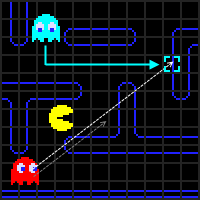
\includegraphics[scale=0.6]{inky-targeting.png}
  \caption{tyrkysový duch}
  \cite{2.zdroj}
\end{figure}
\subsubsection{Oranžový duch(Clyde)}\label{or}
Clyde odchádza z domčeku, ako posledný.V prvých troch leveloch Clyde vôbec nevychádza z domčeka. Jeho rozhodovanie je v celku unikátne a môže sa zdať, že si robí čo chce. Zaujímavá vlastnosť je, že Clyde má dva módy vyberania cieľovej dlaždice, ktoré strieda, podľa toho, ako je blízko Pac-Mana. Keď sa Clyde nachádza viacej, ako 8 dlaždíc od Pac-Mana, tak jeho cieľová dlaždica je ako Blinkyho, presná pozícia Pac-Mana. V momente ako sa Clyde priblíží bližšie, ako 8 dlaždíc jeho cieľová dlaždica je roh bludiska. Kvôli tomuto typu správania vieme Clyda zacikliť, tak aby sa nás nevedel nikdy dotknúť.Na obrázku\ref{oc} nižšie, sú X označené miesta kde Clyde mení svoje režimi. Ak sa Pac-Manovi podarí aby stál na miesťe, tak Clyde sa bude točiť okolo oblasťi v tvare T do nekonečna.\cite{2.zdroj}
\begin{figure}[h!]
  \centering
  \begin{subfigure}[b]{0.4\linewidth}
    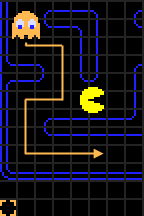
\includegraphics[scale=0.35]{clyde-targeting.png}
    \caption{Clydova cieľova dlaždica.}
\cite{2.zdroj}
  \end{subfigure}
  \begin{subfigure}[b]{0.4\linewidth}
    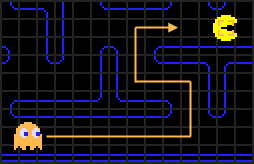
\includegraphics[scale=0.35]{clyde-targeting2.png}
    \caption{Clydova cieľova dlaždica.}
\cite{2.zdroj}
  \end{subfigure}
\begin{subfigure}[b]{0.4\linewidth}
    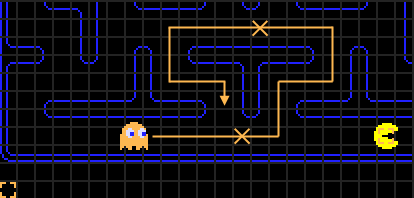
\includegraphics[scale=0.35]{clyde-targeting3.png}
    \caption{Clydova cieľova dlaždica zaciklenie.}
\cite{2.zdroj}
\label{oc}
  \end{subfigure}
\end{figure}
\newpage
\section{Záver}
Prvé umelé inteligencie boli pôvodne len fantáziou, ale vďaka pokroku v počítačových technológiách sa stali skutočnosťou.Tieto systémy boli schopné vykonávať práce, ktoré boli nudné pre ľudí alebo príliš ťažké.
Prvé umelé inteligencia boli použité v hrách už v 60. rokoch minulého storočia. Od vtedy sa neprestali vyvíjať. Vytvárali pre nás prostredia, postavy a úlohy, ktoré zapríčinili to, že sme sa vžili do danej situácie. Umelé inteligencie nemusia byť náročné na to aby splnili svoj účel stačí im iba pár pravidiel alebo skrípt na to aby nás dokázali vtiahnuť do ich sveta.
Napríklad hra Pac-Man patrí medzi prvé hry, v ktorých sa použila umelá inteligencia na správanie sa príšer. Táto jednoduchá umelá inteligencia bola schopná vytvárať reálne správanie príšer, a tým zvýšiť zábavnosť hry. Aj keď sa umelá inteligencia v hre Pac-Man zdá byť jednoduchá, stala sa základom pre vývoj umelých inteligencií v hrách. Dnes sa umelé inteligencie používajú vo väčšine hier a sú schopné vykonávať oveľa komplexnejšie úlohy. V budúcnosti sa očakáva, že umelé inteligencie budú hrať stále dôležitejšiu úlohu v hrách a prinesú nové možnosti pre ich vývojárov a hráčov.

\section{Vyjadrenie k prednáškam}
\subsection{Vizualizácia }
Vizualizácia je proces prezentovania dát pomocou grafických alebo obrazových prvkov, ako sú napríklad slajdy, diagramy, mapy alebo grafy. Týmto spôsobom sa dá ľahšie porozumieť a interpretovať informácie, a tiež z nich vyvodiť závery. Vizualizácia môže byť užitočná pre rôzne účely, ako napríklad pre zobrazenie výsledkov výskumu, pre prezentáciu podnikových dát alebo pre pomoc pri rozhodovaní. Existuje mnoho rôznych spôsobov a nástrojov pre vizualizácia dát, ako napríklad tabuľky, grafy alebo mapy 
\subsection{Bibliografia a citovanie v technickom texte}
Bibliografia je zoznam literatúry, ktorú som použil pri písaní textu. Zvyčajne sa uvádza na konci textu a mal by obsahovať dôležité informácie o každom zdroji, ako sú meno autora, názov diela, vydavateľstvo a dátum vydania. Citovanie je proces, pri ktorom sa odkazujete na prácu iného autora v texte a uvádzame presnú referenciu na túto prácu v bibliografii.
\subsection{Ako napísať technický článok}
Ak chceme napísať technický článok, je dôležité aby sme mali dobrú predstavu o tom, o čom chceme písať. Technické články sa zvyčajne zaoberajú technológiami a je dôležité, aby sme boli oboznámení s týmito témami. Pred začatím písania je dobré si naplánovať, o čom bude článok a, ako ho rozdelíme na jednotlivé časti. Môžeme napríklad začať úvodom, v ktorom vysvetlíme o čom bude článok. Potom môžeme pokračovať konkrétnymi informáciami a príkladmi, ktoré budú podporovať naše tvrdenia. Na konci môžme zhrnúť hlavné body článku a navrhnúť ďalšie možnosti pre výskum alebo čo od budúcnosti očakávame.
\newpage

\bibliography{literatura}
\bibliographystyle{plain} % prípadne alpha, abbrv alebo hociktorý iný

\end{document}
